% Options for packages loaded elsewhere
% Options for packages loaded elsewhere
\PassOptionsToPackage{unicode}{hyperref}
\PassOptionsToPackage{hyphens}{url}
\PassOptionsToPackage{dvipsnames,svgnames,x11names}{xcolor}
%
\documentclass[
  letterpaper,
  DIV=11,
  numbers=noendperiod]{scrartcl}
\usepackage{xcolor}
\usepackage{amsmath,amssymb}
\setcounter{secnumdepth}{-\maxdimen} % remove section numbering
\usepackage{iftex}
\ifPDFTeX
  \usepackage[T1]{fontenc}
  \usepackage[utf8]{inputenc}
  \usepackage{textcomp} % provide euro and other symbols
\else % if luatex or xetex
  \usepackage{unicode-math} % this also loads fontspec
  \defaultfontfeatures{Scale=MatchLowercase}
  \defaultfontfeatures[\rmfamily]{Ligatures=TeX,Scale=1}
\fi
\usepackage{lmodern}
\ifPDFTeX\else
  % xetex/luatex font selection
\fi
% Use upquote if available, for straight quotes in verbatim environments
\IfFileExists{upquote.sty}{\usepackage{upquote}}{}
\IfFileExists{microtype.sty}{% use microtype if available
  \usepackage[]{microtype}
  \UseMicrotypeSet[protrusion]{basicmath} % disable protrusion for tt fonts
}{}
\makeatletter
\@ifundefined{KOMAClassName}{% if non-KOMA class
  \IfFileExists{parskip.sty}{%
    \usepackage{parskip}
  }{% else
    \setlength{\parindent}{0pt}
    \setlength{\parskip}{6pt plus 2pt minus 1pt}}
}{% if KOMA class
  \KOMAoptions{parskip=half}}
\makeatother
% Make \paragraph and \subparagraph free-standing
\makeatletter
\ifx\paragraph\undefined\else
  \let\oldparagraph\paragraph
  \renewcommand{\paragraph}{
    \@ifstar
      \xxxParagraphStar
      \xxxParagraphNoStar
  }
  \newcommand{\xxxParagraphStar}[1]{\oldparagraph*{#1}\mbox{}}
  \newcommand{\xxxParagraphNoStar}[1]{\oldparagraph{#1}\mbox{}}
\fi
\ifx\subparagraph\undefined\else
  \let\oldsubparagraph\subparagraph
  \renewcommand{\subparagraph}{
    \@ifstar
      \xxxSubParagraphStar
      \xxxSubParagraphNoStar
  }
  \newcommand{\xxxSubParagraphStar}[1]{\oldsubparagraph*{#1}\mbox{}}
  \newcommand{\xxxSubParagraphNoStar}[1]{\oldsubparagraph{#1}\mbox{}}
\fi
\makeatother

\usepackage{color}
\usepackage{fancyvrb}
\newcommand{\VerbBar}{|}
\newcommand{\VERB}{\Verb[commandchars=\\\{\}]}
\DefineVerbatimEnvironment{Highlighting}{Verbatim}{commandchars=\\\{\}}
% Add ',fontsize=\small' for more characters per line
\usepackage{framed}
\definecolor{shadecolor}{RGB}{241,243,245}
\newenvironment{Shaded}{\begin{snugshade}}{\end{snugshade}}
\newcommand{\AlertTok}[1]{\textcolor[rgb]{0.68,0.00,0.00}{#1}}
\newcommand{\AnnotationTok}[1]{\textcolor[rgb]{0.37,0.37,0.37}{#1}}
\newcommand{\AttributeTok}[1]{\textcolor[rgb]{0.40,0.45,0.13}{#1}}
\newcommand{\BaseNTok}[1]{\textcolor[rgb]{0.68,0.00,0.00}{#1}}
\newcommand{\BuiltInTok}[1]{\textcolor[rgb]{0.00,0.23,0.31}{#1}}
\newcommand{\CharTok}[1]{\textcolor[rgb]{0.13,0.47,0.30}{#1}}
\newcommand{\CommentTok}[1]{\textcolor[rgb]{0.37,0.37,0.37}{#1}}
\newcommand{\CommentVarTok}[1]{\textcolor[rgb]{0.37,0.37,0.37}{\textit{#1}}}
\newcommand{\ConstantTok}[1]{\textcolor[rgb]{0.56,0.35,0.01}{#1}}
\newcommand{\ControlFlowTok}[1]{\textcolor[rgb]{0.00,0.23,0.31}{\textbf{#1}}}
\newcommand{\DataTypeTok}[1]{\textcolor[rgb]{0.68,0.00,0.00}{#1}}
\newcommand{\DecValTok}[1]{\textcolor[rgb]{0.68,0.00,0.00}{#1}}
\newcommand{\DocumentationTok}[1]{\textcolor[rgb]{0.37,0.37,0.37}{\textit{#1}}}
\newcommand{\ErrorTok}[1]{\textcolor[rgb]{0.68,0.00,0.00}{#1}}
\newcommand{\ExtensionTok}[1]{\textcolor[rgb]{0.00,0.23,0.31}{#1}}
\newcommand{\FloatTok}[1]{\textcolor[rgb]{0.68,0.00,0.00}{#1}}
\newcommand{\FunctionTok}[1]{\textcolor[rgb]{0.28,0.35,0.67}{#1}}
\newcommand{\ImportTok}[1]{\textcolor[rgb]{0.00,0.46,0.62}{#1}}
\newcommand{\InformationTok}[1]{\textcolor[rgb]{0.37,0.37,0.37}{#1}}
\newcommand{\KeywordTok}[1]{\textcolor[rgb]{0.00,0.23,0.31}{\textbf{#1}}}
\newcommand{\NormalTok}[1]{\textcolor[rgb]{0.00,0.23,0.31}{#1}}
\newcommand{\OperatorTok}[1]{\textcolor[rgb]{0.37,0.37,0.37}{#1}}
\newcommand{\OtherTok}[1]{\textcolor[rgb]{0.00,0.23,0.31}{#1}}
\newcommand{\PreprocessorTok}[1]{\textcolor[rgb]{0.68,0.00,0.00}{#1}}
\newcommand{\RegionMarkerTok}[1]{\textcolor[rgb]{0.00,0.23,0.31}{#1}}
\newcommand{\SpecialCharTok}[1]{\textcolor[rgb]{0.37,0.37,0.37}{#1}}
\newcommand{\SpecialStringTok}[1]{\textcolor[rgb]{0.13,0.47,0.30}{#1}}
\newcommand{\StringTok}[1]{\textcolor[rgb]{0.13,0.47,0.30}{#1}}
\newcommand{\VariableTok}[1]{\textcolor[rgb]{0.07,0.07,0.07}{#1}}
\newcommand{\VerbatimStringTok}[1]{\textcolor[rgb]{0.13,0.47,0.30}{#1}}
\newcommand{\WarningTok}[1]{\textcolor[rgb]{0.37,0.37,0.37}{\textit{#1}}}

\usepackage{longtable,booktabs,array}
\usepackage{calc} % for calculating minipage widths
% Correct order of tables after \paragraph or \subparagraph
\usepackage{etoolbox}
\makeatletter
\patchcmd\longtable{\par}{\if@noskipsec\mbox{}\fi\par}{}{}
\makeatother
% Allow footnotes in longtable head/foot
\IfFileExists{footnotehyper.sty}{\usepackage{footnotehyper}}{\usepackage{footnote}}
\makesavenoteenv{longtable}
\usepackage{graphicx}
\makeatletter
\newsavebox\pandoc@box
\newcommand*\pandocbounded[1]{% scales image to fit in text height/width
  \sbox\pandoc@box{#1}%
  \Gscale@div\@tempa{\textheight}{\dimexpr\ht\pandoc@box+\dp\pandoc@box\relax}%
  \Gscale@div\@tempb{\linewidth}{\wd\pandoc@box}%
  \ifdim\@tempb\p@<\@tempa\p@\let\@tempa\@tempb\fi% select the smaller of both
  \ifdim\@tempa\p@<\p@\scalebox{\@tempa}{\usebox\pandoc@box}%
  \else\usebox{\pandoc@box}%
  \fi%
}
% Set default figure placement to htbp
\def\fps@figure{htbp}
\makeatother





\setlength{\emergencystretch}{3em} % prevent overfull lines

\providecommand{\tightlist}{%
  \setlength{\itemsep}{0pt}\setlength{\parskip}{0pt}}



 


\KOMAoption{captions}{tableheading}
\makeatletter
\@ifpackageloaded{caption}{}{\usepackage{caption}}
\AtBeginDocument{%
\ifdefined\contentsname
  \renewcommand*\contentsname{Table of contents}
\else
  \newcommand\contentsname{Table of contents}
\fi
\ifdefined\listfigurename
  \renewcommand*\listfigurename{List of Figures}
\else
  \newcommand\listfigurename{List of Figures}
\fi
\ifdefined\listtablename
  \renewcommand*\listtablename{List of Tables}
\else
  \newcommand\listtablename{List of Tables}
\fi
\ifdefined\figurename
  \renewcommand*\figurename{Figure}
\else
  \newcommand\figurename{Figure}
\fi
\ifdefined\tablename
  \renewcommand*\tablename{Table}
\else
  \newcommand\tablename{Table}
\fi
}
\@ifpackageloaded{float}{}{\usepackage{float}}
\floatstyle{ruled}
\@ifundefined{c@chapter}{\newfloat{codelisting}{h}{lop}}{\newfloat{codelisting}{h}{lop}[chapter]}
\floatname{codelisting}{Listing}
\newcommand*\listoflistings{\listof{codelisting}{List of Listings}}
\makeatother
\makeatletter
\makeatother
\makeatletter
\@ifpackageloaded{caption}{}{\usepackage{caption}}
\@ifpackageloaded{subcaption}{}{\usepackage{subcaption}}
\makeatother
\usepackage{bookmark}
\IfFileExists{xurl.sty}{\usepackage{xurl}}{} % add URL line breaks if available
\urlstyle{same}
\hypersetup{
  pdftitle={Class 6},
  colorlinks=true,
  linkcolor={blue},
  filecolor={Maroon},
  citecolor={Blue},
  urlcolor={Blue},
  pdfcreator={LaTeX via pandoc}}


\title{Class 6}
\author{}
\date{}
\begin{document}
\maketitle


\begin{quote}
Indent
\end{quote}

\textbf{bold}

\emph{italics}

\textbf{Q1: Write a function add() to add some numbers together. Make
sure to add comment(s) to the function explaining why you do things.a.
Your first version of the function should add two input numbers
together; e.g.~add(4, 7) should return 11. {[}1 pt{]}}

\begin{Shaded}
\begin{Highlighting}[]
\NormalTok{add\_2}\OtherTok{\textless{}{-}}\ControlFlowTok{function}\NormalTok{(x,y) \{}
  \CommentTok{\#Adding variables x and y}
\NormalTok{  x}\SpecialCharTok{+}\NormalTok{y}
\NormalTok{\}}
\end{Highlighting}
\end{Shaded}

Testing my function:

\begin{Shaded}
\begin{Highlighting}[]
\FunctionTok{add\_2}\NormalTok{(}\DecValTok{5}\NormalTok{,}\DecValTok{7}\NormalTok{)}
\end{Highlighting}
\end{Shaded}

\begin{verbatim}
[1] 12
\end{verbatim}

\begin{Shaded}
\begin{Highlighting}[]
\FunctionTok{add\_2}\NormalTok{(}\DecValTok{1020293}\NormalTok{,}\DecValTok{20329320}\NormalTok{)}
\end{Highlighting}
\end{Shaded}

\begin{verbatim}
[1] 21349613
\end{verbatim}

Making function with R-studio help

\begin{Shaded}
\begin{Highlighting}[]
\NormalTok{add\_two }\OtherTok{\textless{}{-}} \ControlFlowTok{function}\NormalTok{(x, y) \{}
\NormalTok{  x}\SpecialCharTok{+}\NormalTok{y}
\NormalTok{\}}
\end{Highlighting}
\end{Shaded}

\begin{Shaded}
\begin{Highlighting}[]
\FunctionTok{add\_two}\NormalTok{(}\AttributeTok{x=}\DecValTok{5}\NormalTok{, }\AttributeTok{y=}\DecValTok{9}\NormalTok{)}
\end{Highlighting}
\end{Shaded}

\begin{verbatim}
[1] 14
\end{verbatim}

\textbf{Q1 b. Your second version of the function should add any numbers
together that the user inputs; e.g.~add(1, 2, 3, -4) should return 2.}

\begin{Shaded}
\begin{Highlighting}[]
\NormalTok{add\_multi}\OtherTok{\textless{}{-}}\ControlFlowTok{function}\NormalTok{(x,...)\{}
  \CommentTok{\#Using sum because adding multiple numbers }
  \FunctionTok{sum}\NormalTok{(x,...)}
\NormalTok{\}}

\FunctionTok{add\_multi}\NormalTok{(}\DecValTok{1}\NormalTok{,}\DecValTok{2}\NormalTok{,}\DecValTok{3}\NormalTok{,}\SpecialCharTok{{-}}\DecValTok{4}\NormalTok{)}
\end{Highlighting}
\end{Shaded}

\begin{verbatim}
[1] 2
\end{verbatim}

\begin{Shaded}
\begin{Highlighting}[]
\NormalTok{add\_multi2}\OtherTok{\textless{}{-}}\ControlFlowTok{function}\NormalTok{(x,...) \{}
  \FunctionTok{sum}\NormalTok{(x,...)}
\NormalTok{\}}
\end{Highlighting}
\end{Shaded}

\textbf{Q2: Write a function generate\_dna() that generates a random DNA
sequence of a length input by the user; e.g.~generate\_dna(11) may
return ``ATTTAAGGCTG''. Make sure to add comments to the function. Play
with functions sample() and paste() in your R-Studio Console to see how
they can help here.}

\begin{Shaded}
\begin{Highlighting}[]
\NormalTok{generate\_dna }\OtherTok{\textless{}{-}} \ControlFlowTok{function}\NormalTok{(x) \{}
  \CommentTok{\#Generating a nucleotide vector }
\NormalTok{  nucs }\OtherTok{\textless{}{-}} \FunctionTok{c}\NormalTok{(}\StringTok{"A"}\NormalTok{, }\StringTok{"T"}\NormalTok{, }\StringTok{"G"}\NormalTok{,}\StringTok{"C"}\NormalTok{)}
  \CommentTok{\#Using sample to pull out random nucleotides}
\NormalTok{  nucs\_vector }\OtherTok{\textless{}{-}} \FunctionTok{sample}\NormalTok{ (nucs, x, }\AttributeTok{replace=}\ConstantTok{TRUE}\NormalTok{)}
  \CommentTok{\#Generating a dna string from nucs\_vector}
  \FunctionTok{paste}\NormalTok{(nucs\_vector, }\AttributeTok{collapse=}\StringTok{""}\NormalTok{)}
\NormalTok{\}}

\CommentTok{\#Testing my generate\_data() function }
\FunctionTok{generate\_dna}\NormalTok{(}\DecValTok{34}\NormalTok{)}
\end{Highlighting}
\end{Shaded}

\begin{verbatim}
[1] "TAATACGAAGTTGTATCTTGTCTGCGTTAACGTG"
\end{verbatim}

\textbf{Q3: Write a function generate\_protein() that generates a random
peptide/protein sequence of a length input by the user;
e.g.~generate\_protein(6) may return ``WQRTAG''. Make sure to use the
single-letter code for all 20 amino acids and use no other letters (see
list of amino acids at the bottom of the page); make sure that
individual amino acids can appear more than once. Make sure to add
comments to the function.}

\begin{Shaded}
\begin{Highlighting}[]
\NormalTok{generate\_protein }\OtherTok{\textless{}{-}} \ControlFlowTok{function}\NormalTok{(x)\{}
  \CommentTok{\#Generating a amino acid vector with all 20 amino acids}
\NormalTok{  amino\_acids }\OtherTok{\textless{}{-}} \FunctionTok{c}\NormalTok{(}\StringTok{"A"}\NormalTok{, }\StringTok{"R"}\NormalTok{, }\StringTok{"N"}\NormalTok{, }\StringTok{"D"}\NormalTok{, }\StringTok{"C"}\NormalTok{, }\StringTok{"E"}\NormalTok{, }\StringTok{"Q"}\NormalTok{, }\StringTok{"G"}\NormalTok{, }\StringTok{"H"}\NormalTok{, }\StringTok{"I"}\NormalTok{, }\StringTok{"L"}\NormalTok{, }\StringTok{"K"}\NormalTok{, }\StringTok{"M"}\NormalTok{, }\StringTok{"F"}\NormalTok{, }\StringTok{"P"}\NormalTok{, }\StringTok{"S"}\NormalTok{, }\StringTok{"T"}\NormalTok{, }\StringTok{"W"}\NormalTok{, }\StringTok{"Y"}\NormalTok{,}\StringTok{"V"}\NormalTok{)}
  \CommentTok{\#Using sample to pull out random amino acids}
\NormalTok{  protein\_vector }\OtherTok{\textless{}{-}} \FunctionTok{sample}\NormalTok{(amino\_acids, x, }\AttributeTok{replace=}\ConstantTok{TRUE}\NormalTok{)}
  \CommentTok{\#Generating a protein string from protein\_vector}
  \FunctionTok{paste}\NormalTok{(protein\_vector, }\AttributeTok{collapse=}\StringTok{""}\NormalTok{)}
\NormalTok{\}}
\CommentTok{\#Testing my generate\_protein function}
\FunctionTok{generate\_protein}\NormalTok{(}\DecValTok{6}\NormalTok{)}
\end{Highlighting}
\end{Shaded}

\begin{verbatim}
[1] "RDILEA"
\end{verbatim}

\textbf{Q4: Use your generate\_protein() function to generate peptides
of lengths 5, 7, 9, and 11 amino acids. Take advantage of the base R
function sapply() for this.}

\begin{Shaded}
\begin{Highlighting}[]
\CommentTok{\#Generating vector for peptide lengths}
\NormalTok{lengths }\OtherTok{\textless{}{-}} \FunctionTok{c}\NormalTok{(}\DecValTok{5}\NormalTok{,}\DecValTok{7}\NormalTok{,}\DecValTok{9}\NormalTok{,}\DecValTok{11}\NormalTok{)}
\CommentTok{\#Using sapply to generate peptides for each length}
\NormalTok{peptides }\OtherTok{\textless{}{-}} \FunctionTok{sapply}\NormalTok{(lengths, }\ControlFlowTok{function}\NormalTok{(x) }\FunctionTok{generate\_protein}\NormalTok{(x))}
\CommentTok{\#Displaying the peptides}
\NormalTok{peptides}
\end{Highlighting}
\end{Shaded}

\begin{verbatim}
[1] "DSGQY"       "MLFVAFP"     "SHYGKQFVE"   "WFSPFYTSPFI"
\end{verbatim}

\textbf{Q5: Take each of your peptides from Q4 and run a BLASTP search
(https://blast.ncbi.nlm.nih.gov/Blast.cgi) selecting the Non-redundant
protein sequences (nr) database and homo sapiens (taxid: 9606) organism.
For each search, before clicking BLAST check the Show results in a new
window tab next to the BLAST button to easily allow you to run the blast
search for all four peptides at the same time in four different tabs.
Once each search is done, for the top aligned protein for each peptide,
list the percent identity (Per. Ident) times coverage (Query Cover) (for
example, in the example below, 100\% Query Cover times 85.71\% Per.
Ident = 100\% x 85.71\% = 1.00 x 0.8571 x 100\% = 85.71\%); make sure to
type out your calculations in your Quarto document {[}note: if any of
your values are below 30\% you are probably miscalculating something{]}.
Upload your numbers for each peptide (length (aa) and max identity (\%))
into the shared class excel data sheet (see Data Sheet link in the
Canvas assignment). Also, for each datapoint, add your initials in the
``Your\_Initials'' column of the data sheet. Before adding your
initials, scan through other used initials; if anyone has the same
initials as you, modify your initials to make them unique (your initials
will be used below to identify your specific data points in a ggplot
graph).}

\begin{Shaded}
\begin{Highlighting}[]
\CommentTok{\#Peptide Sequence: VFPYF, Length\_aa: 5, Query cover: 100\%, Percent Identity: 100\%, Percent Identity X Query Cover: 1.00 * 1.00 * 100 = 100\%}
\CommentTok{\#Peptide Sequence: GDVPQKH, Length\_aa: 7, Query cover: 100\%, Percent Identity: 71.43\%, Percent Identity X Query Cover: 1.00 * 0.7143 * 100 = 71.43\%}
\CommentTok{\#Peptide Sequence: HNLKNESWE, Length\_aa: 9, Query cover: 89\%, Percent Identity: 85.71\%, Percent Identity X Query Cover: 0.89 * 0.8571 * 100 = 76.28\%}
\CommentTok{\#Peptide Sequence: PEMEGKCAWMK, Length\_aa: 11, Query cover: 73\%, Percent Identity: 87.50\%, Percent Identity X Query Cover: 0.73 * 0.8750 * 100 = 63.88\%}
\end{Highlighting}
\end{Shaded}

\textbf{Q6: Once there is a good amount of data in the shared excel
sheet, export the sheet as a CSV UTF-8 file (Export option under the
File tab) and save the file to your class working folder (i.e.~the
folder in which you are currently generating a Quarto document). In
R-Studio, upload the csv file into a data frame using the command
peptide\_df \textless- read.csv(``your\_filename''). Use the head()
function to list the first 10 rows (note that the default for head() is
6) of the peptide\_df dataframe as a test that everything looks good.}

\begin{Shaded}
\begin{Highlighting}[]
\CommentTok{\#Using read.csv to pull in the CSV file as a dataframe}
\NormalTok{peptide\_df }\OtherTok{\textless{}{-}} \FunctionTok{read.csv}\NormalTok{(}\StringTok{"BIMM 143 Class 6.csv"}\NormalTok{)}
\CommentTok{\#Displaying the first 10 rows to check the data}
\FunctionTok{head}\NormalTok{(peptide\_df, }\DecValTok{10}\NormalTok{)}
\end{Highlighting}
\end{Shaded}

\begin{verbatim}
   Length_aa Max_Identity_perc Your_Initials  X X.1 X.2 X.3 X.4 X.5 X.6 X.7 X.8
1          5               100           JLA NA  NA  NA  NA  NA  NA  NA  NA  NA
2          7             85.71           JLA NA  NA  NA  NA  NA  NA  NA  NA  NA
3          9             66.85           JLA NA  NA  NA  NA  NA  NA  NA  NA  NA
4         11                55           JLA NA  NA  NA  NA  NA  NA  NA  NA  NA
5          5                80           SKB NA  NA  NA  NA  NA  NA  NA  NA  NA
6          7             85.71           SKB NA  NA  NA  NA  NA  NA  NA  NA  NA
7          9             66.85           SKB NA  NA  NA  NA  NA  NA  NA  NA  NA
8         11                64           SKB NA  NA  NA  NA  NA  NA  NA  NA  NA
9          5               100           KET NA  NA  NA  NA  NA  NA  NA  NA  NA
10         7             85.71           KET NA  NA  NA  NA  NA  NA  NA  NA  NA
   X.9 X.10 X.11 X.12 X.13 X.14 X.15 X.16 X.17 X.18
1   NA   NA   NA   NA   NA   NA   NA   NA   NA   NA
2   NA   NA   NA   NA   NA   NA   NA   NA   NA   NA
3   NA   NA   NA   NA   NA   NA   NA   NA   NA   NA
4   NA   NA   NA   NA   NA   NA   NA   NA   NA   NA
5   NA   NA   NA   NA   NA   NA   NA   NA   NA   NA
6   NA   NA   NA   NA   NA   NA   NA   NA   NA   NA
7   NA   NA   NA   NA   NA   NA   NA   NA   NA   NA
8   NA   NA   NA   NA   NA   NA   NA   NA   NA   NA
9   NA   NA   NA   NA   NA   NA   NA   NA   NA   NA
10  NA   NA   NA   NA   NA   NA   NA   NA   NA   NA
\end{verbatim}

\textbf{Q7: Use ggplot2 to generate a box plot with Length\_aa on the
x-axis and Max\_Identity\_perc on the y-axis. Since the box plot will
require categorical values for Length\_aa, you may have to specify the
x-axis as as.factor(Length\_aa). Feel free to pretty up the plot by
adding your own x/y-axis labels, graph title, etc using the labs()
function and/or using your favorite theme using a theme() function (see
the data-visualization\_ggplot.pdf cheat sheet in Canvas for options).
Optional: you will reuse this plot a few times below, so your subsequent
coding will be simpler if you assign your box plot to an object such as
`p' (p \textless- ggplot(peptide\_df) +\ldots.etc).}

\begin{Shaded}
\begin{Highlighting}[]
\CommentTok{\#Accessing ggplot2}
\FunctionTok{library}\NormalTok{ (ggplot2)}
\CommentTok{\#Generating box plot and assigning to my\_plot}
\NormalTok{my\_plot }\OtherTok{\textless{}{-}} \FunctionTok{ggplot}\NormalTok{(peptide\_df, }\FunctionTok{aes}\NormalTok{(}\AttributeTok{x=}\FunctionTok{as.factor}\NormalTok{(Length\_aa), }\AttributeTok{y=}\NormalTok{Max\_Identity\_perc)) }\SpecialCharTok{+} \FunctionTok{geom\_boxplot}\NormalTok{() }\SpecialCharTok{+}
  \FunctionTok{labs}\NormalTok{(}\AttributeTok{x=}\StringTok{"Peptide Length (aa)"}\NormalTok{, }
   \AttributeTok{y=} \StringTok{"Max Identity (\%)"}\NormalTok{,}
   \AttributeTok{title=}\StringTok{"Distribution of BLAST Identity Scores by Peptide Length"}\NormalTok{) }\SpecialCharTok{+} \FunctionTok{theme\_minimal}\NormalTok{()}
\CommentTok{\#Testing my\_plot}
\NormalTok{my\_plot}
\end{Highlighting}
\end{Shaded}

\pandocbounded{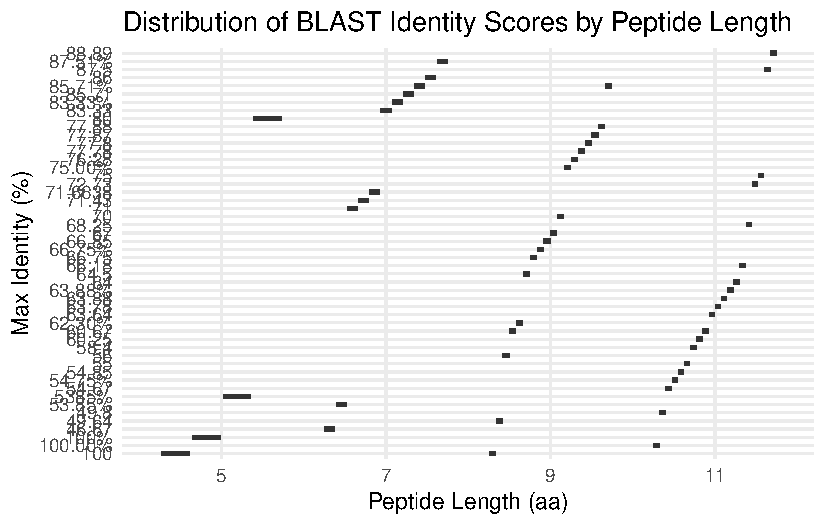
\includegraphics[keepaspectratio]{BIMM-143-Class-6_files/figure-pdf/unnamed-chunk-13-1.pdf}}

\textbf{Q8: Let's add a geom\_jitter() layer to your box plot to
visualize the individual data points on top of the box plot and
highlight your own data points. a. First, add a geom\_jitter() layer to
your box plot with each data point colored according to students'
initials by adding the following additional line to your plot: +
geom\_jitter(aes(col=Your\_Initials)). Feel free to narrow the spread of
the jitter points using the width argument (e.g.~width = 0.2). You can
find your own datapoints this way via the color legend, but it looks
rather messy.}

\begin{Shaded}
\begin{Highlighting}[]
\CommentTok{\#Accessing ggplot2}
\FunctionTok{library}\NormalTok{ (ggplot2)}
\CommentTok{\#Generating box plot and assigning to my\_plot}
\NormalTok{my\_plot }\OtherTok{\textless{}{-}} \FunctionTok{ggplot}\NormalTok{(peptide\_df, }\FunctionTok{aes}\NormalTok{(}\AttributeTok{x=}\FunctionTok{as.factor}\NormalTok{(Length\_aa), }\AttributeTok{y=}\NormalTok{Max\_Identity\_perc)) }\SpecialCharTok{+} \FunctionTok{geom\_boxplot}\NormalTok{() }\SpecialCharTok{+} \FunctionTok{geom\_jitter}\NormalTok{(}\FunctionTok{aes}\NormalTok{(}\AttributeTok{col=}\NormalTok{Your\_Initials), }\AttributeTok{width=}\FloatTok{0.2}\NormalTok{)}
  \FunctionTok{labs}\NormalTok{(}\AttributeTok{x=}\StringTok{"Peptide Length (aa)"}\NormalTok{, }
   \AttributeTok{y=} \StringTok{"Max Identity (\%)"}\NormalTok{,}
   \AttributeTok{title=}\StringTok{"Distribution of BLAST Identity Scores by Peptide Length"}\NormalTok{) }\SpecialCharTok{+} \FunctionTok{theme\_minimal}\NormalTok{()}
\end{Highlighting}
\end{Shaded}

\begin{verbatim}
NULL
\end{verbatim}

\begin{Shaded}
\begin{Highlighting}[]
\CommentTok{\#Testing my\_plot}
\NormalTok{my\_plot}
\end{Highlighting}
\end{Shaded}

\pandocbounded{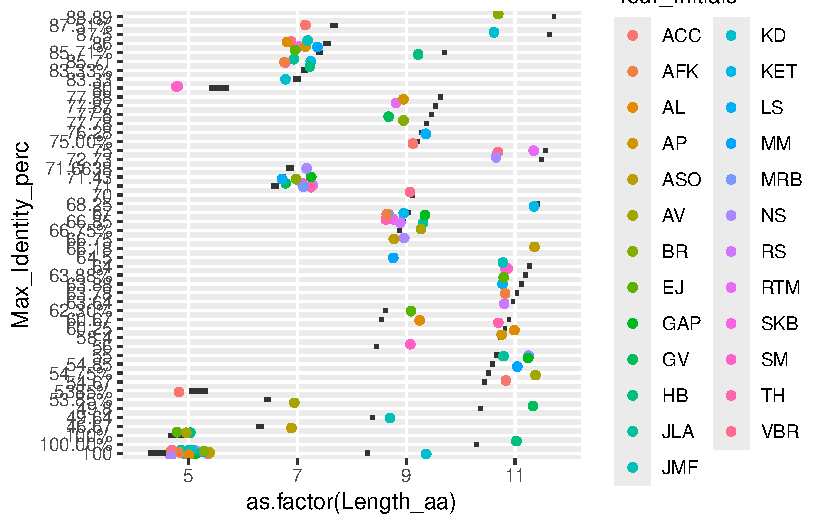
\includegraphics[keepaspectratio]{BIMM-143-Class-6_files/figure-pdf/unnamed-chunk-14-1.pdf}}

\textbf{Q8 b. Now let's control the coloring ourselves to better
highlight your own data points. We can do this by generating a vector
with a color for each datapoint (we will use your favorite color for
your datapoints and ``GREY'' for all other datapoints). You can then use
this vector to assign colors with the geom\_jitter() call.} \textbf{i.
First, use the rep() function to generate a vector consisting of as many
repeats of ``GREY'' as there are datapoints in the peptide\_df data
frame. Assign this vector to an object you name color: i.e.~color
\textless- c(rep(,)) (fill in the blanks). Once you have generated the
color object, use the table() function to ensure that you have the
correct number of instances of ``GREY'' in color. {[}1 pt{]} o Hints for
(i): Use your R-Studio Console to test the outputs of rep(``GREY'', 2),
dim(peptide\_df), and dim(peptide\_df){[}1{]}, and make sure to look at
documentation for the dim() function (?dim) to learn what the output
numbers represent.}

\begin{Shaded}
\begin{Highlighting}[]
\CommentTok{\#Using rep to create GREY for each data point}
\NormalTok{color }\OtherTok{\textless{}{-}} \FunctionTok{c}\NormalTok{(}\FunctionTok{rep}\NormalTok{(}\StringTok{"GREY"}\NormalTok{, }\FunctionTok{dim}\NormalTok{(peptide\_df)[}\DecValTok{1}\NormalTok{]))}
\CommentTok{\#Testing the number of GREY values}
\FunctionTok{table}\NormalTok{(color)}
\end{Highlighting}
\end{Shaded}

\begin{verbatim}
color
GREY 
 100 
\end{verbatim}

\textbf{ii. Next, use the Your\_Initials column in the peptide\_df
dataframe (which can be called as
peptide\_df}\(Your_Initials) to generate a TRUE/FALSE vector indicating which datapoints are yours (TRUE) and which are not (FALSE). Assign this vector to an object you name mydata: i.e. mydata <- _____ (fill in the blank). Again, check that you have the correct number of TRUE and FALSE in mydata using the table() function. [1 pt] o Hint for (ii): Use your R-Studio Console to test the outputs of c("JLA","MK", "BG") == "JLA" and of peptide_df\)Your\_Initials

\begin{Shaded}
\begin{Highlighting}[]
\CommentTok{\#Accessing Your\_Initials column}
\NormalTok{peptide\_df}\SpecialCharTok{$}\NormalTok{Your\_Initials}
\end{Highlighting}
\end{Shaded}

\begin{verbatim}
  [1] "JLA" "JLA" "JLA" "JLA" "SKB" "SKB" "SKB" "SKB" "KET" "KET" "KET" "KET"
 [13] "RTM" "RTM" "RTM" "RTM" "GV"  "GV"  "GV"  "GV"  "RS"  "RS"  "RS"  "RS" 
 [25] "LS"  "LS"  "LS"  "LS"  "TH"  "TH"  "TH"  "TH"  "SM"  "SM"  "SM"  "SM" 
 [37] "AP"  "AP"  "AP"  "AP"  "ASO" "ASO" "ASO" "ASO" "MRB" "MRB" "MRB" "MRB"
 [49] "VBR" "VBR" "VBR" "VBR" "GAP" "GAP" "GAP" "GAP" "MM"  "MM"  "MM"  "MM" 
 [61] "BR"  "BR"  "BR"  "BR"  "AFK" "AFK" "AFK" "AFK" "KD"  "KD"  "KD"  "KD" 
 [73] "NS"  "NS"  "NS"  "NS"  "EJ"  "EJ"  "EJ"  "EJ"  "HB"  "HB"  "HB"  "HB" 
 [85] "AV"  "AV"  "AV"  "AV"  "ACC" "ACC" "ACC" "ACC" "JMF" "JMF" "JMF" "JMF"
 [97] "AL"  "AL"  "AL"  "AL" 
\end{verbatim}

\begin{Shaded}
\begin{Highlighting}[]
\CommentTok{\#Using initials to identify my data points}
\NormalTok{mydata }\OtherTok{\textless{}{-}}\NormalTok{ peptide\_df}\SpecialCharTok{$}\NormalTok{Your\_Initials}\SpecialCharTok{==}\StringTok{"LS"}
\CommentTok{\#Using table with TRUE and FALSE to see how many data points I have}
\FunctionTok{table}\NormalTok{(mydata)}
\end{Highlighting}
\end{Shaded}

\begin{verbatim}
mydata
FALSE  TRUE 
   96     4 
\end{verbatim}

\textbf{iii. Now, use the mydata vector to replace the ``GREY'' values
in the color vector that correspond to your data points with your
favorite color, like this: color{[}mydata{]} \textless- ``COLOR''
(replace ``COLOR'' with the name of your favorite color; see link at the
bottom of the page to a webpage with 657 R color names to select a cool
color). Note, this will replace ``GREY'' with your favorite color for
all the positions that are TRUE in mydata, i.e.~the positions of your
data points. Again, check the vector with table().}

\begin{Shaded}
\begin{Highlighting}[]
\CommentTok{\#Using mydata to change my points to pink}
\NormalTok{color[mydata] }\OtherTok{\textless{}{-}} \StringTok{"pink"}
\CommentTok{\#Testing updated color values}
\FunctionTok{table}\NormalTok{(color)}
\end{Highlighting}
\end{Shaded}

\begin{verbatim}
color
GREY pink 
  96    4 
\end{verbatim}

\textbf{iv.Now you are ready to remake the plot by adding the following
line to your original box plot from Q7: + geom\_jitter(col=color). (Note
that the color call is not run as an aesthetic here because we are now
directly telling ggplot what color to use for each dot). Again, feel
free to use the width argument to narrow the jitter points if you wish
(e.g.~width = 0.2).}

\begin{Shaded}
\begin{Highlighting}[]
\CommentTok{\#Generating final box plot and assigning to my\_plot}
\NormalTok{my\_plot }\OtherTok{\textless{}{-}} \FunctionTok{ggplot}\NormalTok{(peptide\_df, }\FunctionTok{aes}\NormalTok{(}\AttributeTok{x=}\FunctionTok{as.factor}\NormalTok{(Length\_aa), }\AttributeTok{y=}\NormalTok{Max\_Identity\_perc)) }\SpecialCharTok{+} \FunctionTok{geom\_boxplot}\NormalTok{() }\SpecialCharTok{+} \FunctionTok{geom\_jitter}\NormalTok{(}\AttributeTok{col=}\NormalTok{color, }\AttributeTok{width=}\FloatTok{0.2}\NormalTok{) }\SpecialCharTok{+}
  \FunctionTok{labs}\NormalTok{(}\AttributeTok{x=}\StringTok{"Peptide Length (aa)"}\NormalTok{, }
   \AttributeTok{y=} \StringTok{"Max Identity (\%)"}\NormalTok{,}
   \AttributeTok{title=}\StringTok{"Distribution of BLAST Identity Scores by Peptide Length"}\NormalTok{) }\SpecialCharTok{+} \FunctionTok{theme\_minimal}\NormalTok{()}
\CommentTok{\#Testing my\_plot}
\NormalTok{my\_plot}
\end{Highlighting}
\end{Shaded}

\pandocbounded{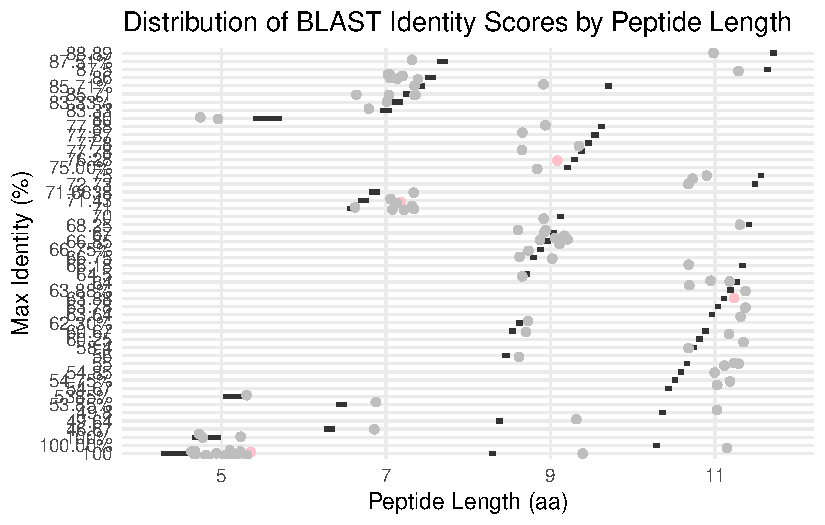
\includegraphics[keepaspectratio]{BIMM-143-Class-6_files/figure-pdf/unnamed-chunk-19-1.pdf}}

\textbf{C. Based on your boxplot, does any of your own peptide data fall
outside the 25 to 75 percentile of the class's data? If yes, list which
one(s).}

Yes, one of my data points, the peptide with length 9 is above the 75th
percentile of the class data.

\textbf{Q9: MHC class II molecules of our immune system display 9 amino
acid peptides on the surface of immune cells that, when from a foreign
origin, activates a T-cell immune response. Based on your findings in Q7
and 8, speculate why those peptides are 9 amino acids long rather than,
say, 5 amino acids.}

As demonstrated on the boxplot, the 9 amino acid peptides have lower
identity and greater variability compared to the 5 amino acids, which
has higher identity and less variability. Therefore, the 9 amino acid
peptides are more distinctive and this increased specifity helps the
immune system distinguish foreign pathogens from itself. MHC class II
molecules display 9 ammino acid peptides because that level of
distinctiveness provides more accurate immune recognition.




\end{document}
